\chapter{Five Skills Every Young Man Should Know}

The source here is an interview rather than a chalkboard lecture, but it still unfolds with a clean internal order. The host introduces Nico Lagan and explains why the conversation matters: he grew up without a male figure, and so the question is how one reconstructs a missing curriculum for young men. The answer comes as a five-part sequence. We are not given a heap of disconnected virtues. We are led, step by step, through an ordered program: protection, courage, provision, temperance, and faith.

Because the lecture offers no board notation, the formulas below are cautious reconstructions of the spoken logic rather than literal transcriptions. The aim is not to force mathematics where none was written, but to preserve the lecture's structure with as much rigor as the source permits.

\section{The Five-Part Order}

The opening promise is explicit: five skills that every young man should master in today's world. The host's autobiographical framing is important. It gives the lecture its tone of repair. We are meant to hear the list as a deliberate curriculum for a life that may otherwise develop by accident.

\begin{definition}
We denote the lecture's ordered five-skill sequence by
\begin{equation}
\Sigma=(\sigma_1,\sigma_2,\sigma_3,\sigma_4,\sigma_5)
=(\mathrm{Protection},\mathrm{Courage},\mathrm{Provision},\mathrm{Temperance},\mathrm{Faith}).
\end{equation}
\end{definition}

The order is part of the argument. Protection comes first because the lecture begins with the body's immediate duties: self-defense and fitness. Courage follows because capacity without action remains inert. Provision widens the frame from self to family. Temperance asks how one governs oneself under pressure. Faith is held back until the end because it marks the boundary of what the speaker thinks can be trained directly.

\begin{remark}
The symbols in this chapter are editorial devices. They do not replace the lecture's spoken language. They merely make the sequence and its internal contrasts easier to hold in view.
\end{remark}

\begin{figure}[h]
\centering
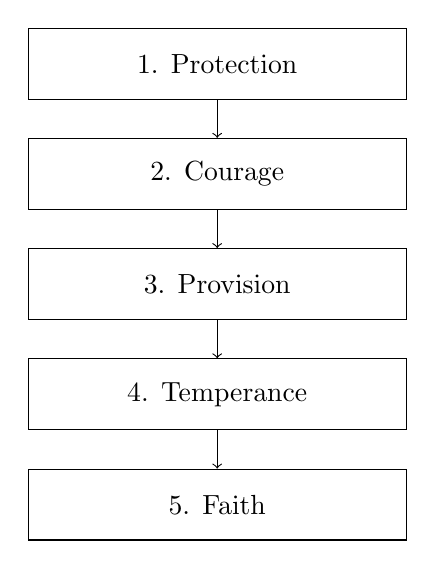
\begin{tikzpicture}
\node[draw, align=center, minimum width=4.8cm, minimum height=0.9cm] (s1) at (0,0) {1. Protection};
\node[draw, align=center, minimum width=4.8cm, minimum height=0.9cm] (s2) at (0,-1.4) {2. Courage};
\node[draw, align=center, minimum width=4.8cm, minimum height=0.9cm] (s3) at (0,-2.8) {3. Provision};
\node[draw, align=center, minimum width=4.8cm, minimum height=0.9cm] (s4) at (0,-4.2) {4. Temperance};
\node[draw, align=center, minimum width=4.8cm, minimum height=0.9cm] (s5) at (0,-5.6) {5. Faith};

\draw[->] (s1.south) -- (s2.north);
\draw[->] (s2.south) -- (s3.north);
\draw[->] (s3.south) -- (s4.north);
\draw[->] (s4.south) -- (s5.north);
\end{tikzpicture}
\caption{The lecture's vertical order. The motion is from bodily competence to action, then to responsibility, self-mastery, and finally belief.}
\end{figure}

\section{Protection: Self-Defense and Bodily Care}

The first skill is protection. Nico does not present this as an abstract ideal. A good man must know how to defend himself, and as part of that same duty he must be physically fit. The lecture deliberately binds self-defense and bodily maintenance together.

We should not move too quickly past the machine analogy that appears here. Nico asks whether we would put bad gas in a car. The point is not biochemical precision. The point is structural. The body is the instrument of protection, and an instrument neglected at the level of fuel, fitness, and upkeep cannot be expected to answer well under pressure. In the lecture's order, fitness is not a decorative bonus to self-defense. It is part of what makes self-defense real.

\subsection{Question \& Answer}

\paragraph{Question.} If martial arts matter, what should a beginner learn first?

\paragraph{Answer.} Nico answers with Muay Thai. He is careful in how he argues. Boxing is not dismissed. It is called simpler, not easier, because it relies only on the fists. Muay Thai is preferred because it enlarges the usable set of tools and adds close-range control.

A compact transcript-based comparison may be written as
\begin{align}
\mathcal{B}_{\mathrm{tools}} &= \{\mathrm{fists}\},\\
\mathcal{M}_{\mathrm{tools}} &= \{\mathrm{fists},\mathrm{elbows},\mathrm{knees},\mathrm{kicks},\mathrm{close\ control}\}.
\end{align}
Within the lecture's restricted comparison we therefore have
\begin{equation}
\mathcal{B}_{\mathrm{tools}} \subsetneq \mathcal{M}_{\mathrm{tools}}.
\end{equation}

This is the practical reason for the recommendation. Boxing leaves the hand to carry the full burden of contact. Nico explicitly adds the real-fight consideration that an unpadded hand may break against a skull. Muay Thai, by contrast, broadens the geometry of available response.

\begin{table}[h]
\centering
\begin{tabular}{|p{0.16\linewidth}|p{0.27\linewidth}|p{0.27\linewidth}|}
\hline
Aspect & Boxing & Muay Thai \\
\hline
Tools named in the lecture & Fists only & Fists, elbows, knees, kicks \\
\hline
Range logic & Punching emphasized & Adds close control \\
\hline
Practical concern & Hand can break on hard contact & More striking options remain available \\
\hline
\end{tabular}
\caption{The lecture's own comparison. Boxing is simpler in tool set; Muay Thai is preferred because it widens the practical repertoire.}
\end{table}

The first skill therefore closes where the lecture wants it to close: not with a vague endorsement of toughness, but with a concrete beginner's recommendation. The host then recaps the first point as self-defense and pivots immediately to the next question: what turns preparation into action?

\section{Courage: When Preparation Crosses into Action}

The second skill is courage. This is the lecture's first major sharpening. Protection gives us capability. Courage asks whether capability ever becomes movement.

Nico's claim is compact and strong. One may have a plan and one may be prepared, but without courage the plan remains inert. In a deliberately schematic notation we may write
\begin{align}
\mathrm{Preparation}\land \neg \mathrm{Courage}
&\Rightarrow
\mathrm{No\ decisive\ action},\\
\mathrm{Preparation}\land \mathrm{Courage}
&\Rightarrow
\mathrm{Action}\to \mathrm{Confidence}.
\end{align}

\begin{proposition}
Within the logic of the lecture, preparation is necessary but not sufficient. Courage is the enabling term that allows preparation to become action.
\end{proposition}

\begin{proof}
The transcript states that many people remain stuck in preparation mode because they are afraid to take the first step. The obstruction is therefore not lack of planning but fear. Once courage enters, the prepared plan becomes executable. Repeated execution then builds confidence, and confidence supports further action.
\end{proof}

What matters here is that courage is not described as the absence of fear. The lecture does not claim that fear vanishes. It claims that fear no longer governs the decision.

\subsection{Question \& Answer}

\paragraph{Question.} Can courage be improved, or is it merely natural?

\paragraph{Answer.} Nico says it can be improved, and he proves the point autobiographically. He describes himself as a bullied child who was afraid. Martial arts then enter the story first as self-defense, then as confidence-building discipline. He says that he went further and stepped into the ring for roughly a dozen amateur fights, frightened each time, in order to prove to himself that he could face an opponent, face fear, and face what life threw at him.

The lecture's internal sequence can be compressed as
\begin{equation}
\mathrm{Fear}\to \mathrm{Training}\to \mathrm{Action\ under\ fear}\to \mathrm{Confidence}.
\end{equation}

We may spell the same pattern out more slowly:
\begin{enumerate}
\item Fear is present.
\item Training increases capability.
\item Capability makes action available.
\item Repeated action under fear builds confidence.
\item Confidence does not abolish fear, but it prevents fear from deciding the outcome.
\end{enumerate}

At this point the lecture has done something important. It has not merely praised courage. It has shown how courage may be formed. That is why the next question naturally concerns mentorship: if courage can be trained, then by whom and under what discipline?

\section{Mentorship and the Search for a Father Figure}

After a brief aside to the audience, the lecture returns with a new problem: for someone who lacks a father figure, where should mentorship be found? The answer begins in the obvious modern place. We are told that we live in a time when one can find examples online, on social media, and on video platforms.

But the lecture refuses to stop there. Nico says that this is not enough. The reason is practical rather than abstract: online appearances may be a front. A persona at a distance can be consumed without transmitting discipline. The answer therefore bends back to martial arts for a third time. Martial arts first appeared as self-defense, then as courage-training, and now they appear as institutions in which coaches function as mentors.

This beat is easy to overlook, but the lecture needs it. Without it, we would jump too abruptly from courage to provision. With it, the argument acquires a social carrier. Character is not only privately declared. It is formed in repeated contact with standards embodied by real people.

\section{Provision: Responsibility Before the Family Arrives}

The third skill is provision. Here the lecture turns outward. The frame is no longer just what a man can do or endure, but what he must supply.

Nico's first move is temporal: one should not wait until a family exists before becoming a provider. The work must start earlier. In a minimal schematic notation,
\begin{equation}
t_{\mathrm{prov\_start}} < t_{\mathrm{family\_formation}}.
\end{equation}

This inequality is simple, but it captures a real shift in the lecture. Provision is not treated as a reaction to circumstance. It is treated as preparation for responsibility.

The lecture then becomes explicitly normative. Nico says that a man should bring money into a relationship and calls this what a man brings ``to the equation.'' The word ``equation'' is rhetorical here, not technical. We should preserve its force without pretending that a formal household model has been derived.

What the lecture is plainly asserting is the following sequence:
\begin{enumerate}
\item provision is a duty rather than an afterthought;
\item provision must begin before family obligations arrive;
\item provision is meant to make care of the family possible.
\end{enumerate}

\begin{remark}
The transcript is garbled in one sentence in this part of the lecture, but the stable claim is clear enough: Nico presents provision as the man's economic responsibility and links it to a division of labor within family life. This should be preserved as his stated norm, not elevated into a general theorem of family economics.
\end{remark}

Once the lecture has named outward responsibility, it immediately asks what inward discipline is needed to carry such responsibility without being ruled by impulse. That is the bridge into temperance.

\section{Temperance: The Control Set and the Traffic Example}

The fourth skill is temperance. Nico glosses it in a stoic register as self-mastery. Here the lecture reaches its clearest formal compression. We are told that there are only three things in life that we control:
\begin{equation}
\mathcal{K}=\{\mathrm{emotions},\mathrm{actions},\mathrm{reactions}\}.
\end{equation}
Everything else belongs outside that set:
\begin{equation}
\mathcal{X}_{\mathrm{external}}=\mathrm{Life}\setminus \mathcal{K}.
\end{equation}

This is a severe partition, and the lecture means it to be severe. We are not being told that external events do not matter. We are being told that they do not obey our will, and that energy wasted on them is misdirected energy. The moral labor of temperance lies in the set \(\mathcal{K}\).

\begin{figure}[h]
\centering
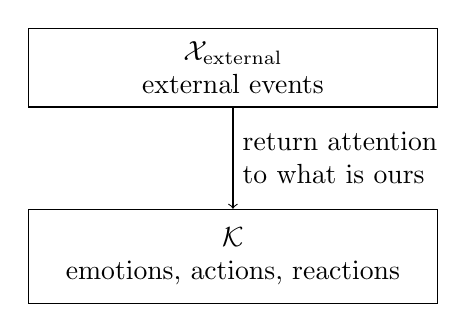
\begin{tikzpicture}
\node[draw, align=center, minimum width=5.2cm, minimum height=1.0cm] (x) at (0,0) {$\mathcal{X}_{\mathrm{external}}$\\external events};
\node[draw, align=center, minimum width=5.2cm, minimum height=1.2cm] (k) at (0,-2.4) {$\mathcal{K}$\\emotions, actions, reactions};
\draw[->] (x.south) -- node[right, align=left] {return attention\\to what is ours} (k.north);
\end{tikzpicture}
\caption{The lecture's stoic partition. What happens to us may lie outside control; what remains ours is the domain of response.}
\end{figure}

\paragraph{Worked example: a driver cuts us off.}
The lecture now tests the partition on a small everyday case. Let \(e\) denote the event of being cut off in traffic, and let \(r\) denote our response. The first classification is immediate:
\begin{align}
e &\in \mathcal{X}_{\mathrm{external}},\\
r &\in \mathcal{K}.
\end{align}
From here the logic branches.

If we react impulsively, the lecture gives an escalation mechanism:
\begin{equation}
e \to r_{\mathrm{impulsive}} \to \mathrm{Escalation} \to \mathrm{Bad\ outcome}.
\end{equation}
If instead we restrain the reaction, the chain is cut:
\begin{equation}
e \to r_{\mathrm{restrained}} \to \mathrm{No\ escalation}.
\end{equation}

We can present the reasoning as a short derivation:
\begin{enumerate}
\item The cut-off is classified as an external event.
\item External events do not move from \(\mathcal{X}_{\mathrm{external}}\) into \(\mathcal{K}\) simply because we dislike them.
\item Our reaction remains inside \(\mathcal{K}\).
\item Therefore the rational intervention point is not the event \(e\), but the response \(r\).
\item Once the response is governed, the escalation chain may be interrupted.
\end{enumerate}

This is why Nico's practical conclusion, ``it doesn't matter,'' should not be read as indifference. It is a rule of attention. It tells us not to surrender control of the only terms that are still ours.

\section{Faith and the Edge of Discipline}

The fifth and final skill is faith. The lecture now reaches its outer boundary. Protection, courage, provision, and temperance have all been treated as disciplines: things we practice, habits we cultivate, domains in which effort matters directly. Faith is placed last because it is introduced as different in kind.

\subsection{Question \& Answer}

\paragraph{Question.} Why does faith belong on the list, and why is it placed at the end?

\paragraph{Answer.} Nico says that faith matters because it is the only one of the five skills that is not under the same kind of direct control as the others. One either believes or one does not. He then gives the answer an inductive extension: if we read enough biographies of great men, we find that they repeatedly had faith in something larger than themselves.

A compact summary of the distinction is
\begin{equation}
\{\sigma_1,\sigma_2,\sigma_3,\sigma_4\}\subseteq \mathcal{T}_{\mathrm{trainable}},
\qquad
\sigma_5\notin \mathcal{D}_{\mathrm{direct\ control}}.
\end{equation}

This is not a metaphysical proof, and it should not be read as one. It is a classification internal to the lecture. The first four skills belong to the domain of disciplined practice. Faith, by contrast, is presented as orientation toward a larger order, whether that order is named as God, the universe, or nature. It comes last because it stands where deliberate training meets its limit.

\section{Summary}

The lecture unfolds as a deliberate progression rather than a list of disconnected slogans. First we are taught protection, because a man must be able to defend himself and maintain the body that carries action. Then we move to courage, because preparation without decisive movement remains sterile. Mentorship enters not as ornament but as the social structure that carries training into character. Provision widens the frame from the self to the family. Temperance sharpens the whole discussion by partitioning life into what lies within control and what does not. Faith closes the sequence by marking the one indispensable orientation that the speaker does not treat as directly trainable.

Taken together, these notes should be read as a transcript-faithful curriculum in responsibility under pressure. The mathematics here is schematic, but it is not empty. It captures the lecture's most disciplined content: an order of skills, a comparison of tool sets, a model of action under fear, a partition of control, and a boundary between practice and belief.